\documentclass{fisatproject}
\title{Hologram with Haptic Feedback}
\team{Leo Varghese \\ Mohit Rajan E\\ Riya Alexander}
\author{Mohit Rajan E}
\begin{document}
\maketitle
\makecert

\newpage
\pagenumbering{roman}
\setcounter{page}{1}
\newgeometry{top=4cm,bottom=0.1cm}
\thispagestyle{plain}
\renewcommand\abstractname{ABSTRACT}
\begin{abstract}
\vspace{5cm}
This paper is intended to analyze and discuss the developments made so far in the field of holography and holographic projection, it discusses the doability and the eventuality in the field of touchable holograms, which works in gear with hand gestures. In this paper, first some elementary matters about what a hologram is and a concise description of how they are devised is discussed. Then how hologram interact with our hand gestures and provide haptic feedback is discussed. In this paper the focus is on the feasibility or doability study of some methods and the analysis and consequences of these methods. Challenges in the whole process will be confronted and then some discussion about future scopes of this technology and where this technology can lead us is done.
\end{abstract}



\newpage
\renewcommand\abstractname{Contribution by Author}
\thispagestyle{plain}
\begin{abstract}
\vspace{5cm}
Author Contribution  Goes Here
\vspace{1cm}
\begin{flushright}
Student Name
\end{flushright}
\end{abstract}

\newpage
\renewcommand\abstractname{ACKNOWLEDGMENT}
\thispagestyle{plain}
\begin{abstract}
\vspace{5cm}
Your Acknowledgement Goes Here
\vspace{1cm}
\begin{flushright}
Student 1
\end{flushright}
\end{abstract}
\newpage

\restoregeometry
\tableofcontents
\newpage

\cleardoublepage
\addcontentsline{toc}{chapter}{\listfigurename}
\listoffigures
\newpage

\cleardoublepage
\addcontentsline{toc}{chapter}{\listtablename}
\listoftables
\newpage



\chapter{Introduction}
\pagenumbering{arabic}
\setcounter{page}{1}
\renewcommand{\baselinestretch}{1.50}
\section{Overview}
\par Haptic holography is a combination of computational modeling and multimodal spatial display.It enables a person to see, feel, and interact with free standing holographic pictures of material surfaces that is three-dimensional in nature. In this paper, various holographic displays are merged with a force-feedback device to render multimodal images with programmatically prescribed material properties and behavior.


\par A method to produce haptic objects in the air using spatial modulation of ultrasound is initiated. Methods of airborne ultrasonic tactile display is based on vibrotactile radiation pressure and sensor feedback systems, which results in low spatial receptive resolution. The initiated approach produces a spatially standing haptic image using stationary ultrasonic waves that enables user to touch 3D images without depending on vibrotactile stimulation and sensor feedback.


\section{Problem Statement}

\par In the current education system students are taught to learn formulas and how to use them but not to reason or understand the logic behind them, causing then to forget it in a short peroid.It is a typical longitudianl learning approah. Our brain system is not just longitudianl in learning process, but much more complex. Current education system evolved on the basis of visual and audotory senses and their application leads to memmorizing the content of learning rather than creaing a holistic perceprtion.
% which can be based on the enormous untapped abilities of the human brain.
It is observed that the current education system  uses mainly audio methods to teach students.
In India around 10\% of students suffer from some form of learning disibility[1]. Research also point to the fact that visual working memory is better in students with learning disibility rather than audority working memory[2].
It can be infered that a modern method of learning should be devloped in order to increase the efficiency of learning process.

\par To addres this issue  we propose a system which uses a hologramic display with haptic feedback by the interaction of using hand gestures. This project will focus on developing a system as described above to introduce a new approch to learn basic geometry.

\section{Objective}

To create a system which also includes somesthetic senses to learning. To achive this a hologramic display with haptic feedback is proposed. The proposed system can be used to project objects in mid-air which can be intracted by using the hand gestures to view new objects, change or modifiy its properties like size, view etc.

\chapter{Literature Review}

The world population is the sum of all humans on Earth. As of today, it is estimated to number 7.004 billion by the United States Census Bureau. The USCB estimates that the world population exceeded 7 billion on March 12, 2012. According to a separate estimate by the United Nations Population Fund, it reached this milestone on October 31, 2011.
\begin{table}[h!]
\begin{center}
\begin{tabular}{|c|c|c|c|}
\hline Rank & Country & Population  & Percentage  \\ 
\hline 1 & China & 1,347,350,000 & 19.24\% \\ 
\hline 2 & India & 1,210,193,422  & 17.28\% \\ 
\hline 3 & United States & 313,269,000 & 4.47\% \\ 
\hline 
\end{tabular}
\caption{World Population Table} 
\end{center}
\end{table}
The world's population is unevenly distributed, with six of Earth's seven continents being permanently inhabited on a large scale. As of 2012, Asia is the most populous continent, with its 4.1 billion inhabitants accounting for over 60\% of the world population. The world's two most-populated countries alone, China and India, constitute about 37\% of the world's population. Africa is the second-most-populated continent, with around 1 billion people, or 15\% of the world's population. Europe's 733 million people make up 11\% of the world's population, while the Latin American and Caribbean regions are home to 589 million (9\%).


\chapter{Design}

The proposed system consist of three sub-systems
\begin{itemize}
    \item  Display
    \item Haptic feedback
    \item Hand gesture regonazing system.
    \item Software compontent ? (is this required?)
\end{itemize}
\subsection{Display}
Hologram was selected as the method of display. Since previous  research has shown learning gemotry with hologram is better than tradional methods[3].

\subsection{Haptic feedback}
Haptic feedback is added to add a somesthetic senses to learning. And also as a response to convay the previous commanf by the user has been registred.

\subsection{Hand Gesture}
Hand Gestures are used as the input to the system and will be used by the user to intract with the system.
{Required bellow part?}
The hand geuster is proccess using Google  MediaPipe libaray.

\section{Proposal}
In mathematics, Stirling's approximation (or Stirling's formula) is an approximation for large factorials. It is named after James Stirling.

The formula as typically used in applications is:

$$
\ln (n!) = n \ln n - n  + O(\ln(n))
$$

\chapter{Work Plan}
    \begin{figure}[h!]
        \begin{center}
        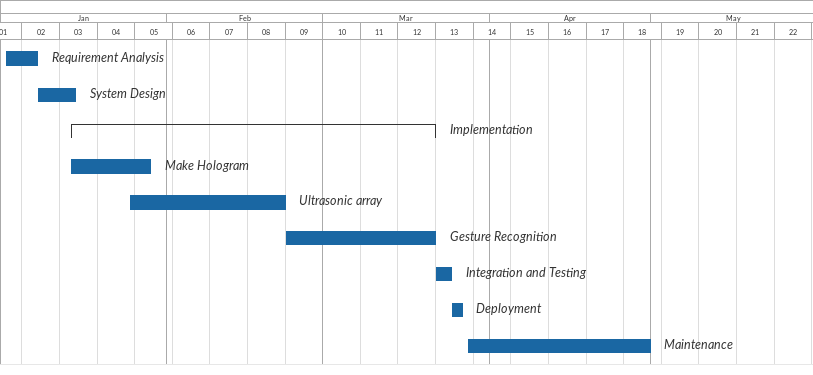
\includegraphics[scale=.6]{images/work_plan.png}
        \caption{Work Plan}
        \end{center}
        \end{figure}
 \section{Budget}
\chapter{Conclusion}

An intrusion detection system (IDS) \cite{nist} is a device or software application that monitors network and/or system activities for malicious activities or policy violations and produces reports to a Management Station.


Donald Ervin Knuth \cite{knuth} is a computer scientist and Professor Emeritus at Stanford University. He is the author of the seminal multi-volume work The Art of Computer Programming. Knuth has been called the "father" of the analysis of algorithms


\begin{thebibliography}{1}
\bibitem{nist} K. Scarfone and P. Mell, ``Guide to intrusion detection and prevention systems
(idps),'' \textit{NIST Special Publication}, vol. 800, no. 2007, p. 94, 2007.
\bibitem{knuth} Wikipedia, ``Donald knuth.'' \url{http://en.wikipedia.org/wiki/Donald_Knuth}.


\end{thebibliography}
\end{document}
